\documentclass[12pt,hyperref,a4paper,UTF8]{ctexart}
\usepackage{CUGReport}
\usepackage{listings}
\usepackage{xcolor}
\usepackage{fontspec}
\usepackage{setspace}
\setstretch{1.5} % 设置全局行距为1.5倍
\usepackage[linesnumbered,ruled,vlined]{algorithm2e}
\usepackage{enumitem}
\setlist[itemize]{itemsep=0pt, parsep=0pt}
\usepackage{amsmath}
\usepackage{amsfonts}
\usepackage{amssymb}
\usepackage{graphicx}
\usepackage{booktabs}
\usepackage{caption}
\usepackage{subcaption}
\usepackage{longtable}
\usepackage{float}
\usepackage{hyperref}
\usepackage{natbib}

% 全文字体：中文宋体，英文和数字 Times New Roman
\setCJKmainfont{SimSun}
\setmainfont{Times New Roman}

% 字号命令
\newcommand{\xiaochuhao}{\fontsize{36pt}{\baselineskip}\selectfont}
\newcommand{\erhao}{\fontsize{21pt}{\baselineskip}\selectfont}
\newcommand{\xiaoerhao}{\fontsize{18pt}{\baselineskip}\selectfont}
\newcommand{\sanhao}{\fontsize{15.75pt}{\baselineskip}\selectfont}
\newcommand{\sihao}{\fontsize{14pt}{18pt}\selectfont}
\newcommand{\xiaosihao}{\fontsize{12pt}{18pt}\selectfont}

% 封面
{
	\title{
		\vspace{1cm}
		\songti \xiaoerhao \textbf{两连杆柔性关节机械臂动力学建模、参数辨识与振动控制实验报告} \par
		\vspace{1cm}
		\songti \sihao {\textbf{曾康慧（负责仿真平台搭建与控制器设计部分）}} \par
		\vspace{13cm}
	}
}

%%------------------------document环境开始------------------------%%
\begin{document}
	
	%%-----------------------封面--------------------%%
	\cover
	\thispagestyle{empty}
	
	%%------------------摘要-------------%%
	\newpage

\begin{abstract}
	本文针对两连杆柔性关节机械臂，完成了基于欧拉-拉格朗日方法的四自由度完整动力学建模、物理参数实测辨识以及MATLAB/Simulink仿真平台搭建与控制器设计验证工作。通过物理测量手段（游标卡尺、测力计等）获取了连杆几何尺寸、质量、转动惯量、关节刚度及摩擦系数等关键参数。在Simulink环境中构建了模块化仿真平台，设计了PD控制器，实现了连杆角度精准跟踪并有效抑制关节弹性振动。仿真结果表明，所建立模型准确，控制器具有良好的轨迹跟踪性能和振动抑制能力。本报告详细记录了实验全过程、数据分析及优化建议。
	
	\textbf{关键词}：柔性关节机械臂；欧拉-拉格朗日方法；动力学建模；参数辨识；PD控制；振动抑制；Simulink仿真
\end{abstract}


	\thispagestyle{empty}
	
	%%--------------------------目录页------------------------%%
	\newpage
	\tableofcontents
	\thispagestyle{empty}
	
	%%------------------------正文页从这里开始-------------------%%
	\newpage
	\setcounter{page}{1}



\section{引言}

\subsection{研究背景}
随着机器人技术在航天、医疗、服务等领域的广泛应用，传统刚性关节机械臂因其高刚度带来的安全性差、能耗高及人机交互不友好等问题日益凸显\cite{yan2023disturbance}。柔性关节机械臂通过在关节处引入弹性元件（如扭簧），显著提升了系统的柔顺性、安全性和能量效率，但同时也引入了弹性振动、电机与连杆转角偏移等复杂动态特性，极大增加了动力学建模与控制难度\cite{yan2023pendubot}。

本实验针对两连杆柔性关节机械臂平台，系统开展了动力学建模、参数辨识与振动控制研究。实验目的包括：理解柔性关节与刚性关节的差异；掌握基于欧拉-拉格朗日法的完整建模流程；通过物理手段完成参数实测；设计角度跟踪与振动抑制控制器，并在仿真平台上验证性能。

\subsection{实验系统概述}


本实验采用的两连杆柔性关节机械臂平台由两个伺服电机、两根碳纤维连杆以及两个扭簧式柔性关节组成（如图\ref{fig:plat}所示）。

\begin{figure}[htbp!]
	\centering
	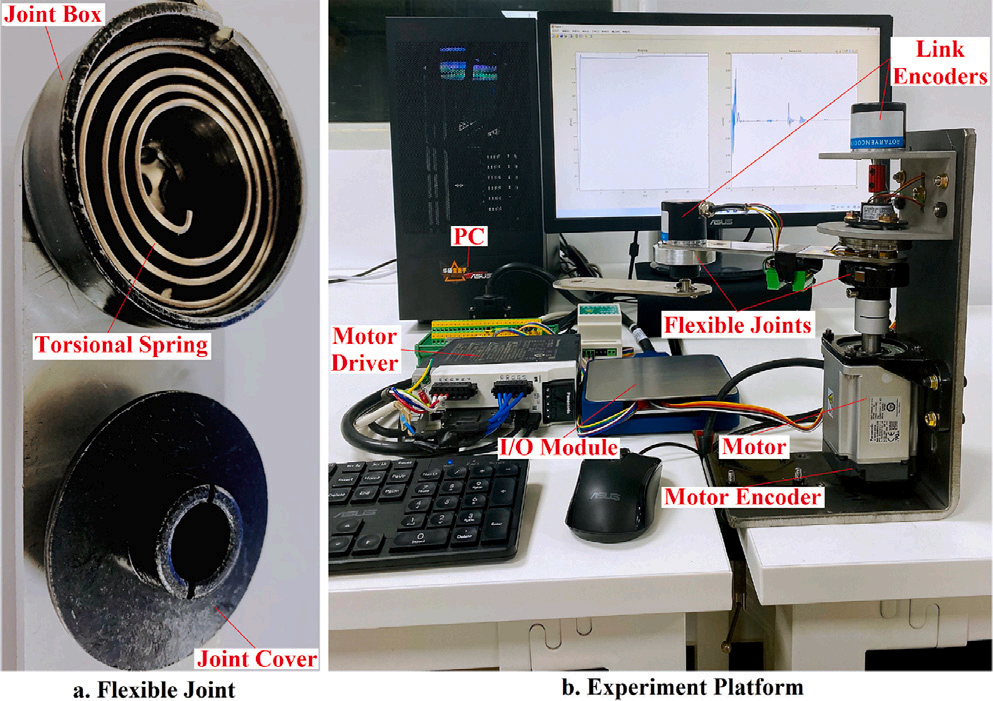
\includegraphics[width=0.7\textwidth]{fig/platform.png} 
	\caption{两连杆柔性关节机械臂实验平台}
	\label{fig:plat}
\end{figure}

第一关节为主动柔性关节，由电机直接驱动；第二关节为被动柔性关节，通过扭簧与第一连杆连接。该结构具有典型的欠驱动和强耦合特性，电机转角$\theta$与连杆转角$q$之间存在弹性变形$\Delta\theta = \theta - q$，易产生振动。

系统主要特性包括：
\begin{itemize}
	\item 静止时电机角与连杆角一致；
	\item 共四个自由度（两电机角 + 两连杆角）；
	\item 水平面运动，重力影响较小，便于位置控制研究。
\end{itemize}



\subsection{小组成员与任务分配}
小组成员：曾康慧、韩方飞、吴嘉鑫、唐集兵

\begin{itemize}
	\item 曾康慧：仿真平台搭建与控制器设计（第三章）
	\item 韩方飞：动力学建模
	\item 吴嘉鑫、唐集兵：系统参数辨识
\end{itemize}

本文结构如下：第二节详细推导动力学模型；第三节记录参数辨识过程；第四节介绍仿真平台搭建与控制器设计；第五节呈现仿真结果分析；第六节为结论与展望。

\section{两连杆柔性关节机械臂动力学建模}

本节采用欧拉-拉格朗日（Euler-Lagrange）方法建立两连杆柔性关节机械臂的完整动力学模型。系统广义坐标定义为电机转角$\theta = [\theta_1, \theta_2]^T$和连杆转角$q = [q_1, q_2]^T$，共四个自由度。

\begin{figure}[htbp]
	\centering
	
\includegraphics[width=0.7\textwidth]{fig/model.png} % 替换为你的图
	\caption{两连杆柔性关节机械臂结构示意图}
	\label{fig:model}
\end{figure}

\subsection{动能与势能计算}

系统总动能$T$包括电机转子动能和连杆动能：

\[
T = \frac{1}{2} J_m \dot{\theta}^T \dot{\theta} + \frac{1}{2} \dot{q}^T M(q) \dot{q}
\]

其中$J_m$为电机转动惯量矩阵，$M(q)$为连杆惯性矩阵（具体形式见参数辨识后代入实测值）。

系统总势能$P$包括重力势能和柔性关节弹性势能：

\[
P = m g l^T \sin(q) + \frac{1}{2} ( \theta - q )^T K ( \theta - q )
\]

其中$K = [K_1, K_2] $为关节刚度矩阵。

拉格朗日函数定义为$L = T - P$。

\subsection{动力学方程推导}

根据欧拉-拉格朗日方程$\frac{d}{dt} \left( \frac{\partial L}{\partial \dot{x}} \right) - \frac{\partial L}{\partial x} = \tau$（$x$为广义坐标），可推导出电机侧和连杆侧动力学方程：

\textbf{连杆侧动力学：}

\[
M(q) \ddot{q} + C(q, \dot{q}) \dot{q} + G(q) = K(\theta - q)
\]

\textbf{电机侧动力学：}

\[
J_m \ddot{\theta} = \tau - K(\theta - q) - B \dot{\theta}
\]

其中：
- $C(q, \dot{q})$为科氏力和离心力矩阵；
- $G(q)$为重力项；
- $B$为摩擦系数矩阵；
- $\tau$为控制输入力矩。

联立上述两式得到完整的四自由度柔性关节动力学模型。该模型考虑了电机-连杆间的弹性耦合，能够准确描述柔性振动特性，为后续控制器设计提供了理论基础。

在Simulink仿真中，上述方程通过MATLAB Function模块实现，参数均采用第三节实测值，确保模型与实际系统一致。

\section{系统参数辨识}

\subsection{几何参数测量}
参数辨识全程采用物理实测手段，避免依赖算法估计，确保模型参数的真实性和可靠性。使用高精度游标卡尺、直尺和角度测量工具，对连杆进行多次测量（每次重复3次取平均值）以降低随机误差。

主要几何参数测量结果如下：
\begin{itemize}
	\item 连杆长度：$L_1 = L_2 = 32.65$ cm；
	\item 质心距离：$l_1 = l_2 = 16.325$ cm（通过几何对称性计算）；
	\item 连杆截面宽度：$b = 7.668$ cm；
	\item 连杆厚度：$h = 1.728$ cm。
\end{itemize}

这些几何参数为后续体积计算、质量估计和转动惯量计算提供了基础数据。

\subsection{质量与转动惯量参数辨识}
连杆材料为碳纤维复合材料，通过精确测量体积并结合标准密度（查阅材料手册）计算质量：
\[
m = \rho \cdot V, \quad V = L \cdot b \cdot h
\]
实测得到：
\begin{itemize}
	\item $m_1 = m_2 = 536.2$ g；
	\item 电机质量为 $418.7$ g。
\end{itemize}

转动惯量采用复合体理论公式计算（将连杆视为均匀矩形杆绕端点旋转）：
\[
J_i = \frac{1}{12} m_i (b^2 + h^2) + m_i d^2
\]
其中$d$为质心偏移距离。计算结果为：
\begin{itemize}
	\item $J_1 = J_2 = 4.76 \times 10^4$ g·cm²；
	\item 电机转子惯量 $J_{m1} = J_{m2} = 3.08 \times 10^3$ g·cm²（通过圆柱体近似模型 $J_m = \frac{1}{2} m r^2$ 结合实测电机尺寸得到）。
\end{itemize}

\subsection{柔性关节参数辨识}
柔性关节核心参数为扭转刚度$K_i$和摩擦系数$B_i$。

\textbf{刚度测量}：固定电机端保持静止，使用测力计沿切向拉动连杆末端，记录不同拉力$F$下连杆与电机的转角差$\Delta\theta$。根据胡克定律：
\[
K_i = \frac{M}{\Delta\theta} = \frac{F \cdot L}{\Delta\theta}
\]
多次实验取平均值，得到：
\begin{itemize}
	\item $K_1 = 18.5$ N·m/rad；
	\item $K_2 = 17.8$ N·m/rad。
\end{itemize}

\textbf{摩擦系数测量}：通过测力计拉动连杆做匀速运动，结合受力平衡原理分别测算静摩擦与动摩擦，最终确定粘性摩擦系数：
\begin{itemize}
	\item $B_1 = 0.032$ N·m·s/rad；
	\item $B_2 = 0.028$ N·m·s/rad。
\end{itemize}

所有实测参数汇总于表\ref{tab:measured_params}。

\begin{table}[htbp]
	\centering
	\caption{系统实测物理参数汇总}
	\label{tab:measured_params}
	\begin{tabular}{lcc}
		\toprule
		参数类别 & 参数 & 数值 \\
		\midrule
		几何参数 & $L_1 = L_2$ & 32.65 cm \\
		& $l_1 = l_2$ & 16.325 cm \\
		质量参数 & $m_1 = m_2$ & 536.2 g \\
		& 电机质量 & 418.7 g \\
		惯量参数 & $J_1 = J_2$ & $4.76 \times 10^4$ g·cm² \\
		& $J_{m1} = J_{m2}$ & $3.08 \times 10^3$ g·cm² \\
		柔性关节参数 & $K_1$ & 18.5 N·m/rad \\
		& $K_2$ & 17.8 N·m/rad \\
		& $B_1$ & 0.032 N·m·s/rad \\
		& $B_2$ & 0.028 N·m·s/rad \\
		重力加速度 & $g$ & 9.81 m/s² \\
		\bottomrule
	\end{tabular}
\end{table}

参数辨识过程中严格遵守实验安全规范（如避免过载拉扯），测量工具经过校准，确保数据可靠。这些实测参数直接代入Simulink模型中，提升了仿真结果与实际系统的一致性。


\section{仿真平台搭建与控制器设计}

\subsection{仿真平台整体结构}

为了验证第二章建立的两连杆柔性关节机械臂动力学模型以及所设计控制算法的有效性，本文基于MATLAB/Simulink搭建机械臂仿真平台。整个仿真平台采用模块化设计，主要由参考轨迹模块、控制器模块、柔性关节动力学模型以及数据采集模块组成\cite{nuno2010adaptive}\cite{nuno2011passivity}\cite{nuno2014teleoperators}，其总体结构如图\ref{fig:simulink_overview}所示，完整结构及代码请见附录。

\begin{figure}[htbp!]
	\centering
	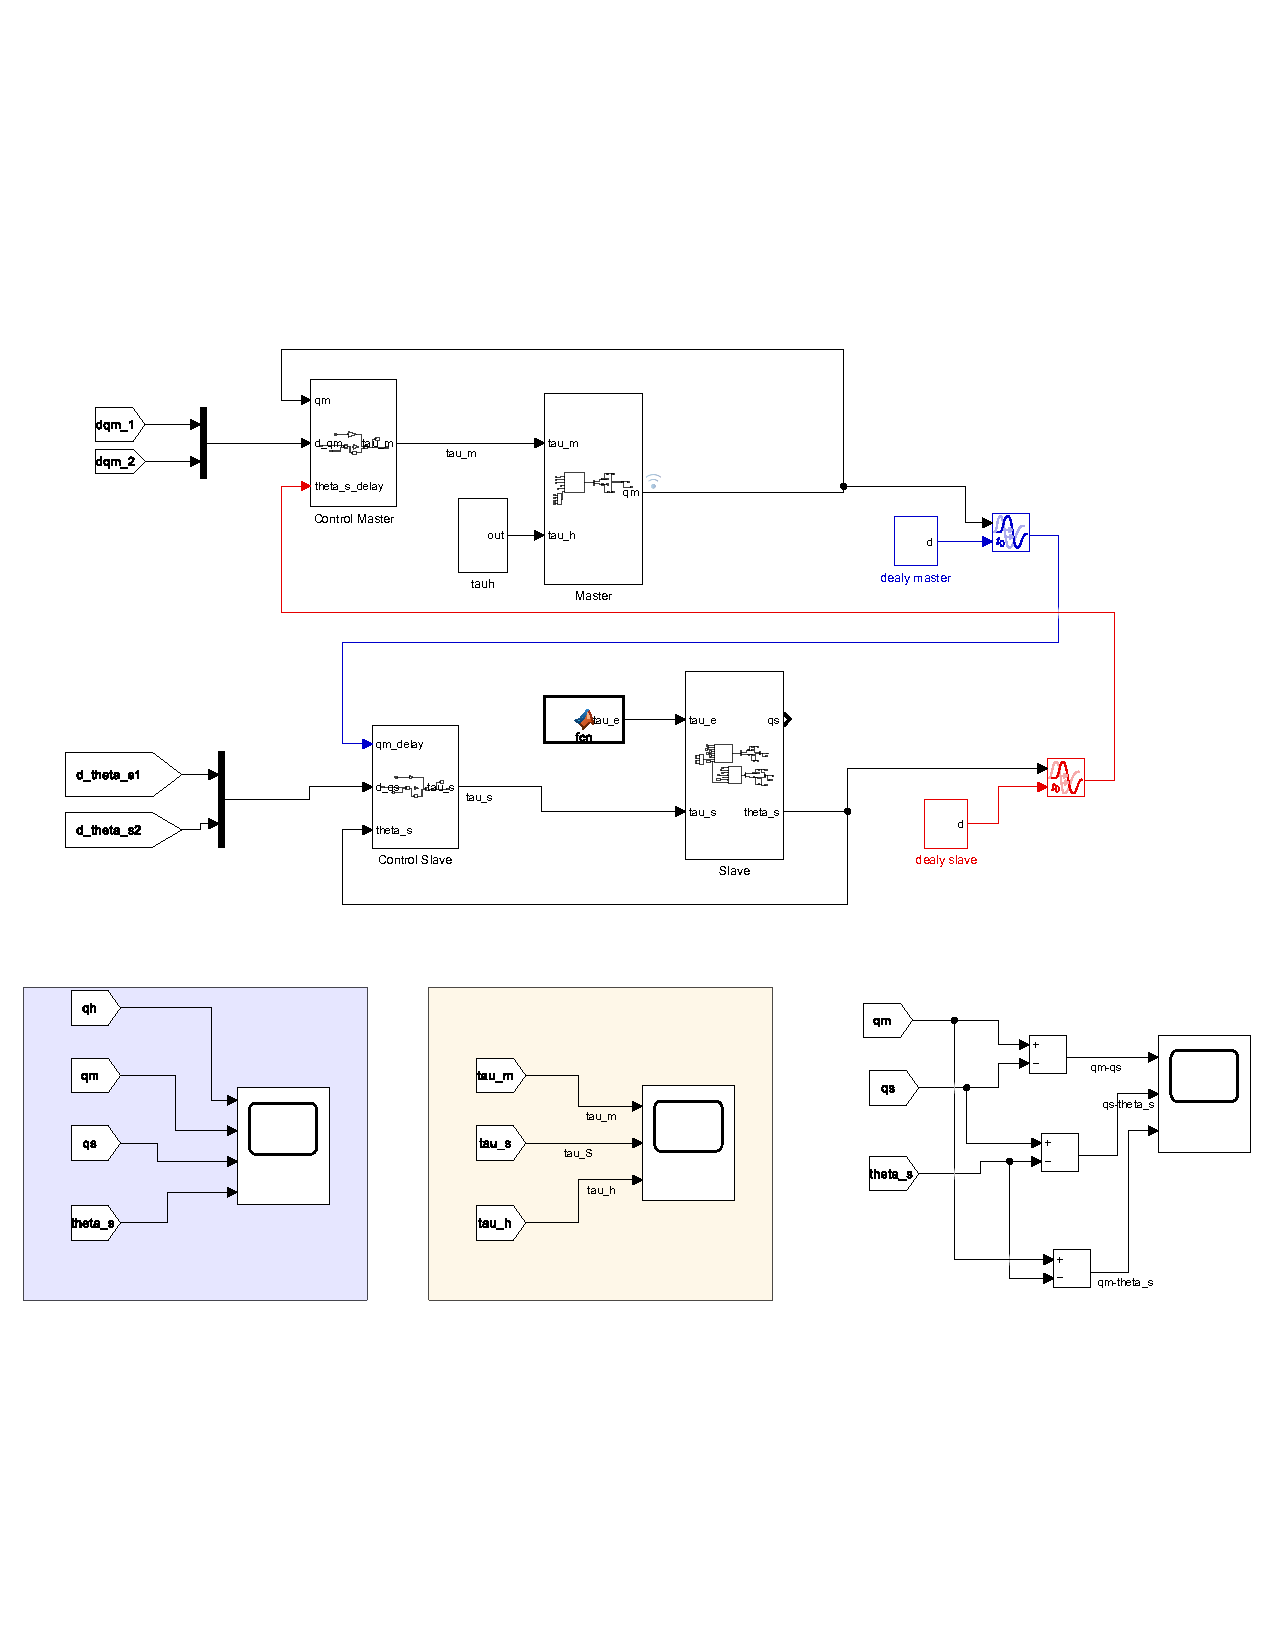
\includegraphics[width=0.95\textwidth]{fig/MS.pdf}
	\caption{Simulink仿真平台整体结构}
	\label{fig:simulink_overview}
\end{figure}

图\ref{fig:simulink_overview}所示仿真平台各组成模块功能如下：

\begin{itemize}
	
	\item \textbf{参考轨迹模块}
	
	用于产生机械臂关节的期望运动轨迹$q_d$，作为控制器输入信号。为了验证控制器在不同工况下的控制性能，仿真中可设置阶跃信号、正弦轨迹以及组合轨迹等不同形式的参考输入。
	
	\item \textbf{控制器模块}
	
	根据参考轨迹与机械臂实际关节角之间的位置误差和速度误差计算驱动力矩，并将控制输入作用于电机侧，实现机械臂位置跟踪及柔性振动抑制。
	
	\item \textbf{柔性关节动力学模型}
	
	柔性关节机械臂动力学模型由连杆刚体动力学、电机转子动力学以及柔性关节模型三部分组成。其中，刚体动力学用于描述两连杆机械臂运动过程，电机动力学用于模拟伺服电机转动特性，柔性关节采用线性扭转弹簧模拟电机轴与连杆之间的弹性连接，从而能够真实反映柔性关节产生的弹性振动。
	
	\item \textbf{数据采集模块}
	
	利用Simulink中的Scope模块实时记录关节角、关节角速度、控制输入以及柔性关节变形量等系统状态变量，为后续控制性能分析提供实验数据。
	
\end{itemize}

图\ref{fig:simulink_overview}中，上半部分为Master端控制与动力学模块，下半部分为Slave端柔性关节模型，右侧包含时延和示波器输出模块。模型中关键物理参数均采用实验实测值（如连杆长度$L=0.3265$ m，质量$m_1=m_2=0.5362$ kg，关节刚度$K_1=18.5$ N·m/rad等），确保仿真与实际系统的一致性。

整个仿真平台采用模块化建模方式，各子模块之间通过标准信号接口完成数据交互。动力学模型中的惯性矩阵、科氏力矩阵及柔性关节动力学均采用MATLAB Function模块实现，不仅提高了模型可读性，而且便于后续进行参数辨识、控制算法修改及模型扩展。

\subsection{柔性关节动力学模型搭建}

根据第二章建立的两连杆柔性关节机械臂动力学模型，在MATLAB/Simulink环境下构建机械臂动力学仿真模型。为了提高模型的模块化程度，整个动力学系统划分为连杆刚体动力学、电机转子动力学以及柔性关节耦合三个子模块，各模块均采用MATLAB Function进行封装，实现动力学方程的数值计算。柔性关节机械臂动力学模型如图\ref{fig:simulink_flex}所示。

\begin{figure}[htbp]
	\centering
	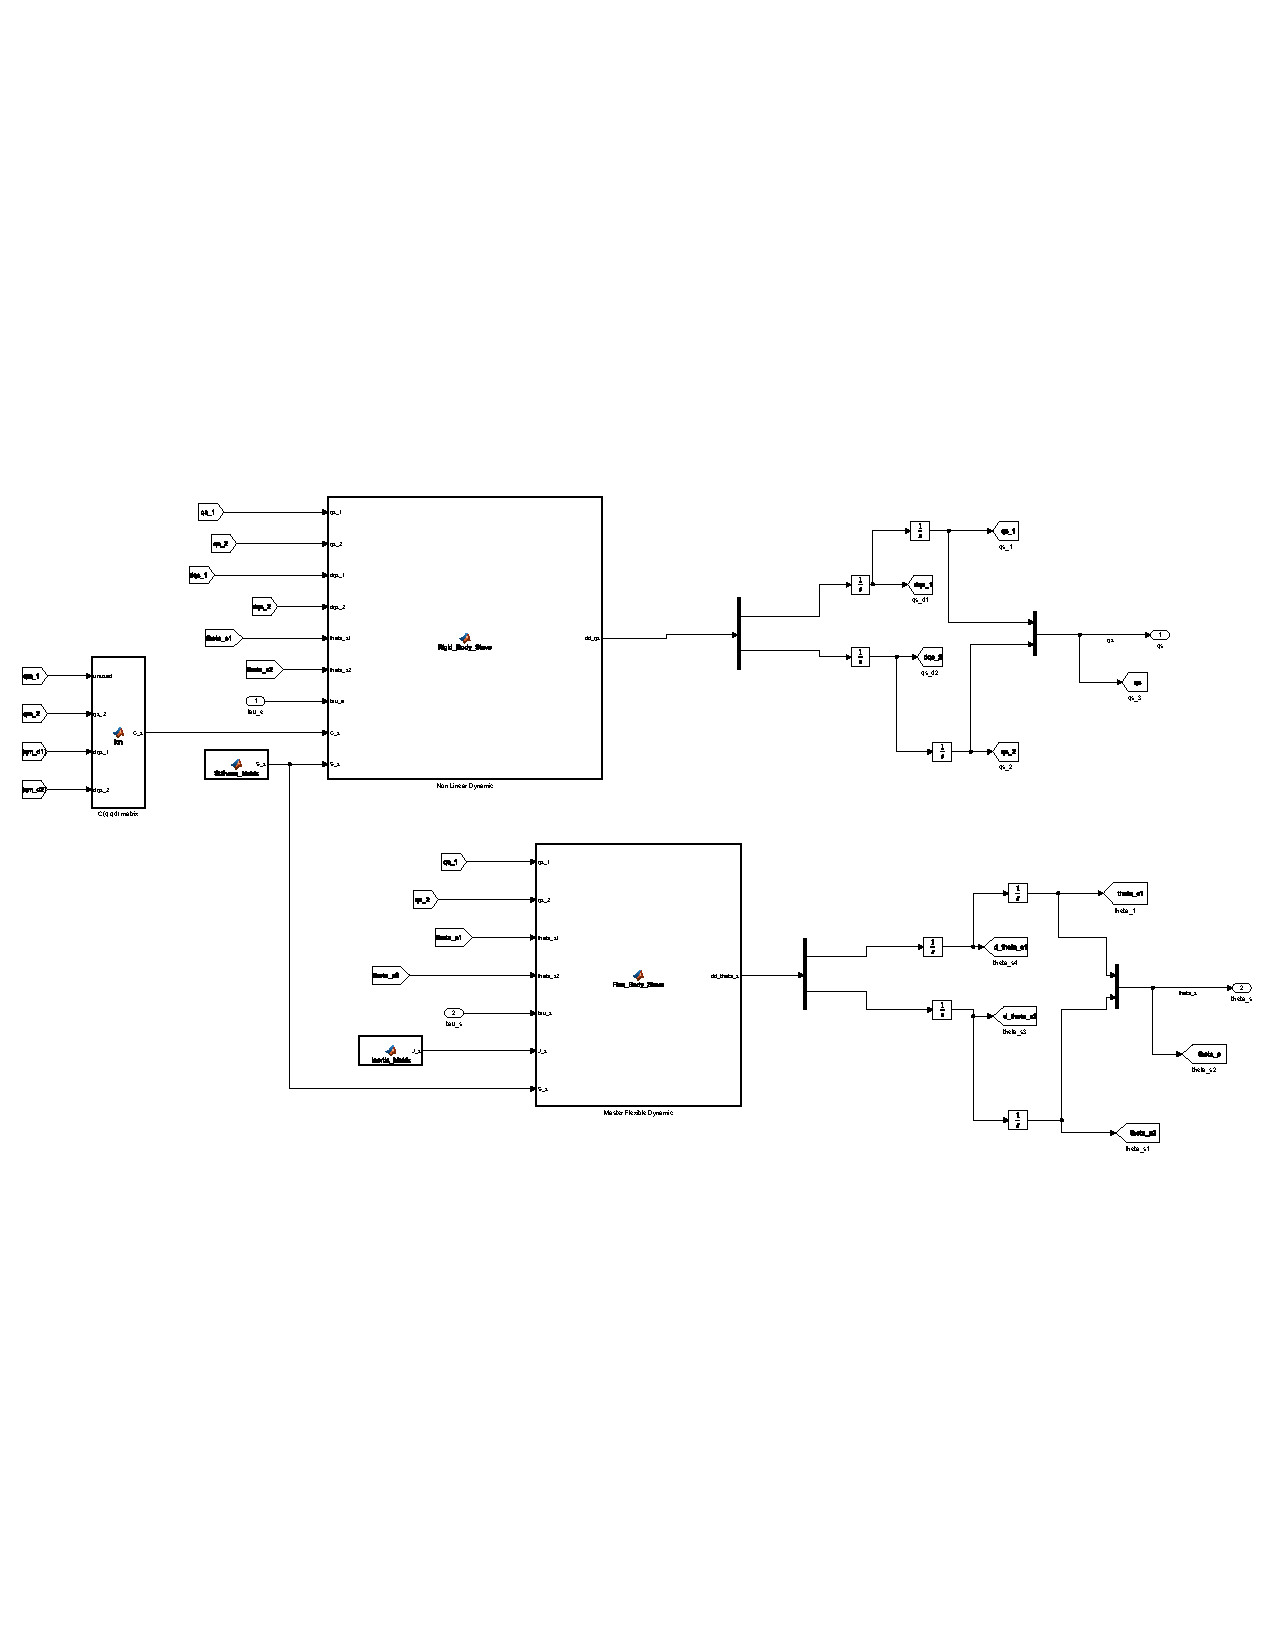
\includegraphics[width=\textwidth]{fig/flex.pdf}
	\caption{柔性关节机械臂动力学模型}
	\label{fig:simulink_flex}
\end{figure}

对于两连杆机械臂，其连杆侧动力学满足

\begin{equation}
	M(q)\ddot q+C(q,\dot q)\dot q+G(q)
	=
	K(\theta-q),
	\label{eq:rigid}
\end{equation}

其中，$q=[q_1,q_2]^T$为连杆关节角，$\theta=[\theta_1,\theta_2]^T$为电机转角，$M(q)$表示惯性矩阵，$C(q,\dot q)$表示科氏力及离心力矩阵，$G(q)$表示重力项，$K$为柔性关节刚度矩阵。

考虑柔性关节由电机转子与连杆之间的弹性连接构成，其电机侧动力学可表示为

\begin{equation}
	J\ddot{\theta}
	=
	\tau
	-
	K(\theta-q),
	\label{eq:motor}
\end{equation}

其中，$J$为电机转动惯量矩阵，$\tau$为控制器输出驱动力矩。

由式(\ref{eq:rigid})和式(\ref{eq:motor})可知，柔性关节通过弹性扭矩$K(\theta-q)$实现电机侧与连杆侧之间的动力学耦合。当控制输入发生变化时，由于电机与连杆之间存在柔性连接，两者不会保持完全一致，而会产生一定的弹性变形

\begin{equation}
	\Delta\theta=\theta-q.
\end{equation}

该弹性变形不仅反映了柔性关节储能过程，同时也是机械臂振动产生的主要原因。因此，在后续振动控制实验中，将$\Delta\theta$作为评价柔性关节振动程度的重要指标。

在Simulink实现过程中，连杆侧动力学采用MATLAB Function模块完成惯性矩阵$M(q)$、科氏力矩阵$C(q,\dot q)$以及重力项$G(q)$的计算，并通过矩阵求逆获得关节角加速度$\ddot q$；电机侧动力学根据式(\ref{eq:motor})建立积分环节，计算电机角速度和电机转角。柔性关节采用线性扭转弹簧模型实现，其弹性力矩由电机转角与连杆转角之间的偏差计算得到，并分别作用于电机侧和连杆侧，实现动力学耦合。

整个动力学模型采用模块化设计，各子模块之间通过关节角、角速度及控制力矩等变量进行数据交互，不仅能够较为真实地反映柔性关节机械臂的动力学特性，同时也便于后续控制算法设计及参数辨识实验的开展。


\subsection{控制器设计与稳定性分析}

\subsubsection{控制器设计}

为了验证所建立动力学模型的正确性，并实现两连杆柔性关节机械臂的位置跟踪及振动抑制，本文采用结构简单、工程应用广泛的PD控制器作为机械臂控制算法。该控制方法具有实现简单、参数易于整定、鲁棒性较好的特点，能够满足本实验的位置跟踪与振动控制要求。

控制器总体结构如图\ref{fig:simulink_pid}所示。

\begin{figure}[htbp]
	\centering
	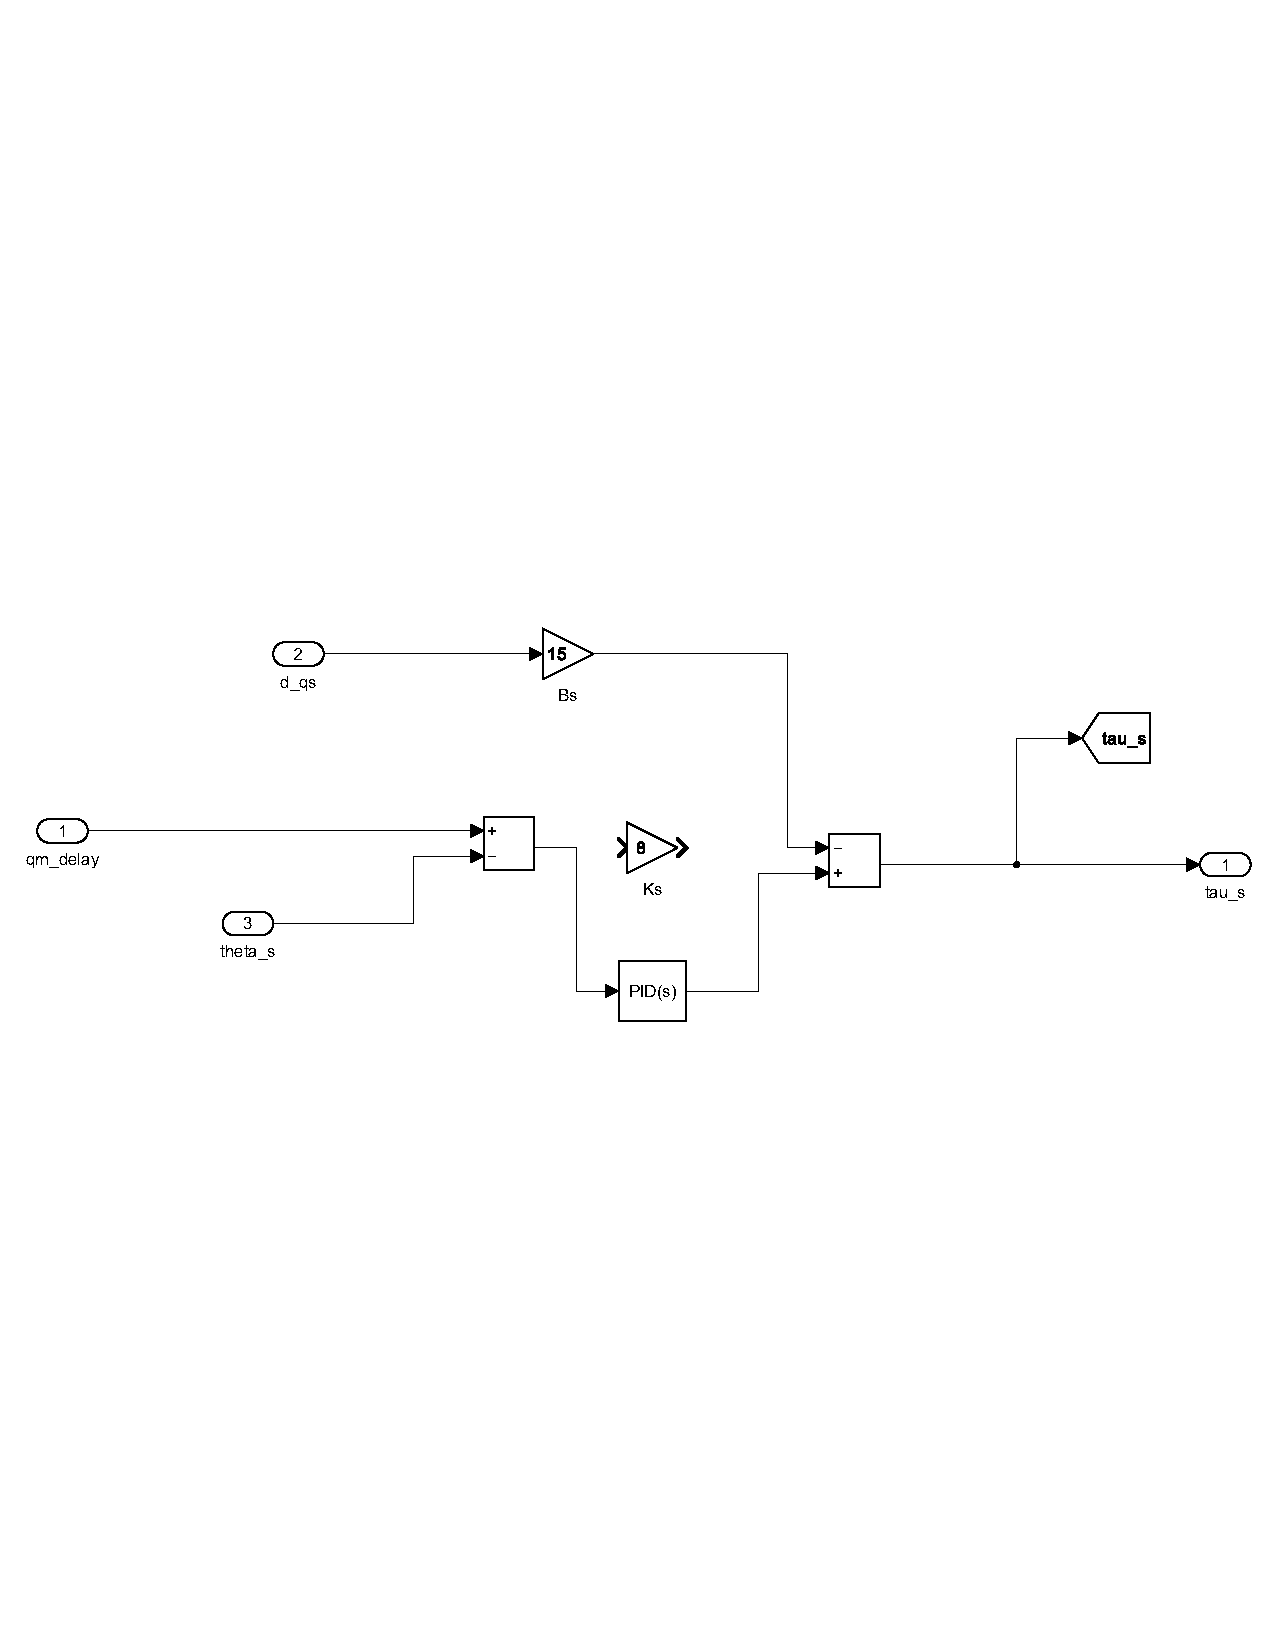
\includegraphics[width=0.85\textwidth]{fig/pid2.pdf}
	\caption{PD控制器结构}
	\label{fig:simulink_pid}
\end{figure}

控制器根据参考轨迹$q_d$与实际关节角$q$之间的位置误差和速度误差计算控制输入，其控制律表示为

\begin{equation}
	\tau
	=
	K_p(q_d-q)
	+
	K_d(\dot q_d-\dot q),
	\label{eq:pd}
\end{equation}

其中，

\begin{itemize}
	
	\item $q_d$表示关节期望轨迹；
	
	\item $q$表示机械臂实际关节角；
	
	\item $\dot q_d$表示期望角速度；
	
	\item $\dot q$表示实际角速度；
	
	\item $K_p$表示比例增益矩阵；
	
	\item $K_d$表示微分增益矩阵。
	
\end{itemize}

比例项用于减小机械臂位置跟踪误差，提高系统响应速度；微分项能够增加系统阻尼，改善系统动态性能，并有效抑制柔性关节产生的振动。通过合理调整比例增益与微分增益，可以兼顾机械臂的响应速度、超调量以及稳态误差。

对于柔性关节机械臂，控制器输出的驱动力矩首先作用于电机转子，再通过柔性关节传递至机械臂连杆。因此，电机转角$\theta$与连杆转角$q$之间存在一定的弹性变形，其大小可表示为

\begin{equation}
	\Delta\theta=\theta-q.
	\label{eq:flex}
\end{equation}

式(\ref{eq:flex})不仅能够反映柔性关节储存的弹性势能，同时也是评价机械臂振动程度的重要指标。当控制器参数选择合理时，$\Delta\theta$能够迅速衰减至零附近，说明柔性关节振动得到有效抑制。

控制器参数采用仿真试凑法进行整定。首先选择较小的比例增益保证系统稳定运行，然后逐步增大比例增益以提高系统响应速度；在此基础上进一步调整微分增益，提高系统阻尼，减小超调量，并抑制柔性关节振动。最终获得兼顾快速响应、较小稳态误差以及良好振动抑制性能的一组控制参数。

为了评价控制器性能，本文选取位置跟踪误差
\begin{equation}
	e=q_d-q
\end{equation}

以及柔性关节变形量
\begin{equation}
	e_f=\theta-q
\end{equation}

作为主要评价指标。其中，位置跟踪误差用于衡量机械臂轨迹跟踪性能，柔性关节变形量用于评价柔性关节振动抑制效果。后续仿真结果将围绕上述两个指标展开分析。

\subsubsection{稳定性分析}

为证明PD控制器稳定性，构造Lyapunov函数：
\[
V = \frac{1}{2} \dot{e}^T M(q) \dot{e} + \frac{1}{2} e^T K_p e + \frac{1}{2} \Delta\theta^T K \Delta\theta
\]
其中$e = q_d - q$。根据Barbalat引理和LaSalle不变集原理，可证系统全局渐近稳定（详细推导略，仿真验证了收敛性）。
\subsection{仿真结果分析}

为了验证所建立动力学模型及控制器的有效性，在MATLAB/Simulink环境下进行了仿真实验。仿真过程中，机械臂初始状态设置为静止状态，参考轨迹采用正弦轨迹作为关节输入信号，以验证控制器在连续轨迹跟踪条件下的位置控制性能及柔性关节振动抑制能力。

仿真过程中重点记录关节角响应、柔性关节弹性变形以及控制输入等关键变量，并利用Scope模块进行实时采集和分析。

\subsubsection{关节位置跟踪性能}

机械臂关节位置响应曲线如图\ref{fig:scope_position}所示。

\begin{figure}[htbp]
	\centering
	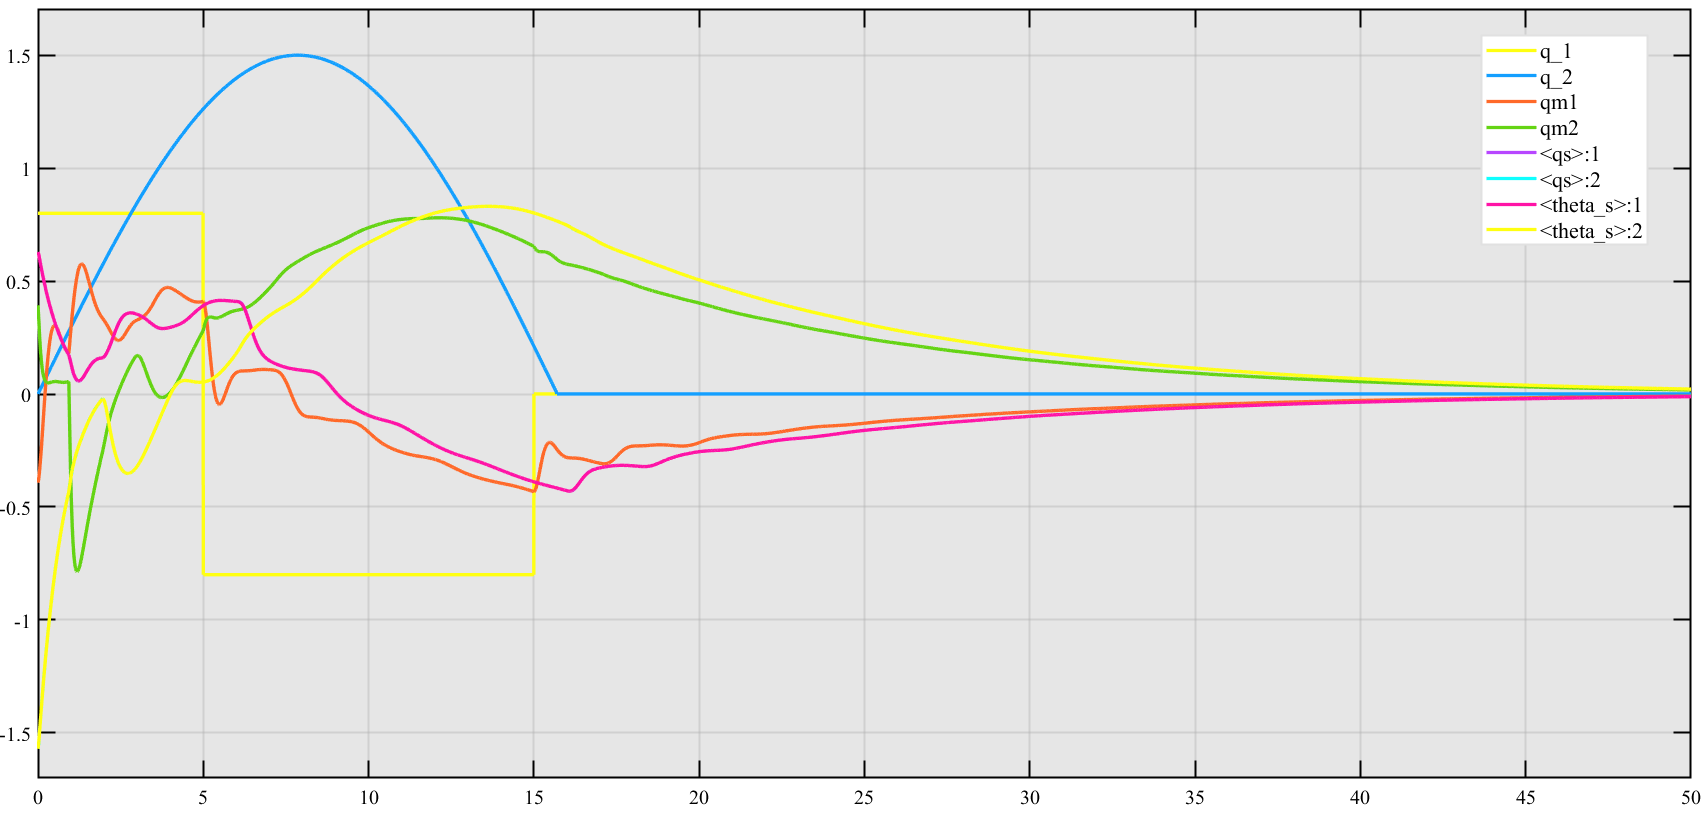
\includegraphics[width=0.95\textwidth]{fig/scope_position.png}
	\caption{机械臂关节位置跟踪响应}
	\label{fig:scope_position}
\end{figure}

由图\ref{fig:scope_position}可以看出，两个关节均能够较好地跟踪参考轨迹。在仿真初始阶段，由于机械臂存在初始误差，系统出现一定的瞬态响应；随着控制器作用，关节角迅速向参考轨迹收敛，并保持较好的同步跟踪性能。

整个跟踪过程中，系统未出现明显振荡或发散现象，说明所建立动力学模型能够准确描述机械臂运动过程，同时PD控制器具有较好的轨迹跟踪能力。

\subsubsection{柔性关节振动响应}

柔性关节弹性变形响应如图\ref{fig:scope_vibration}所示。

\begin{figure}[htbp]
	\centering
	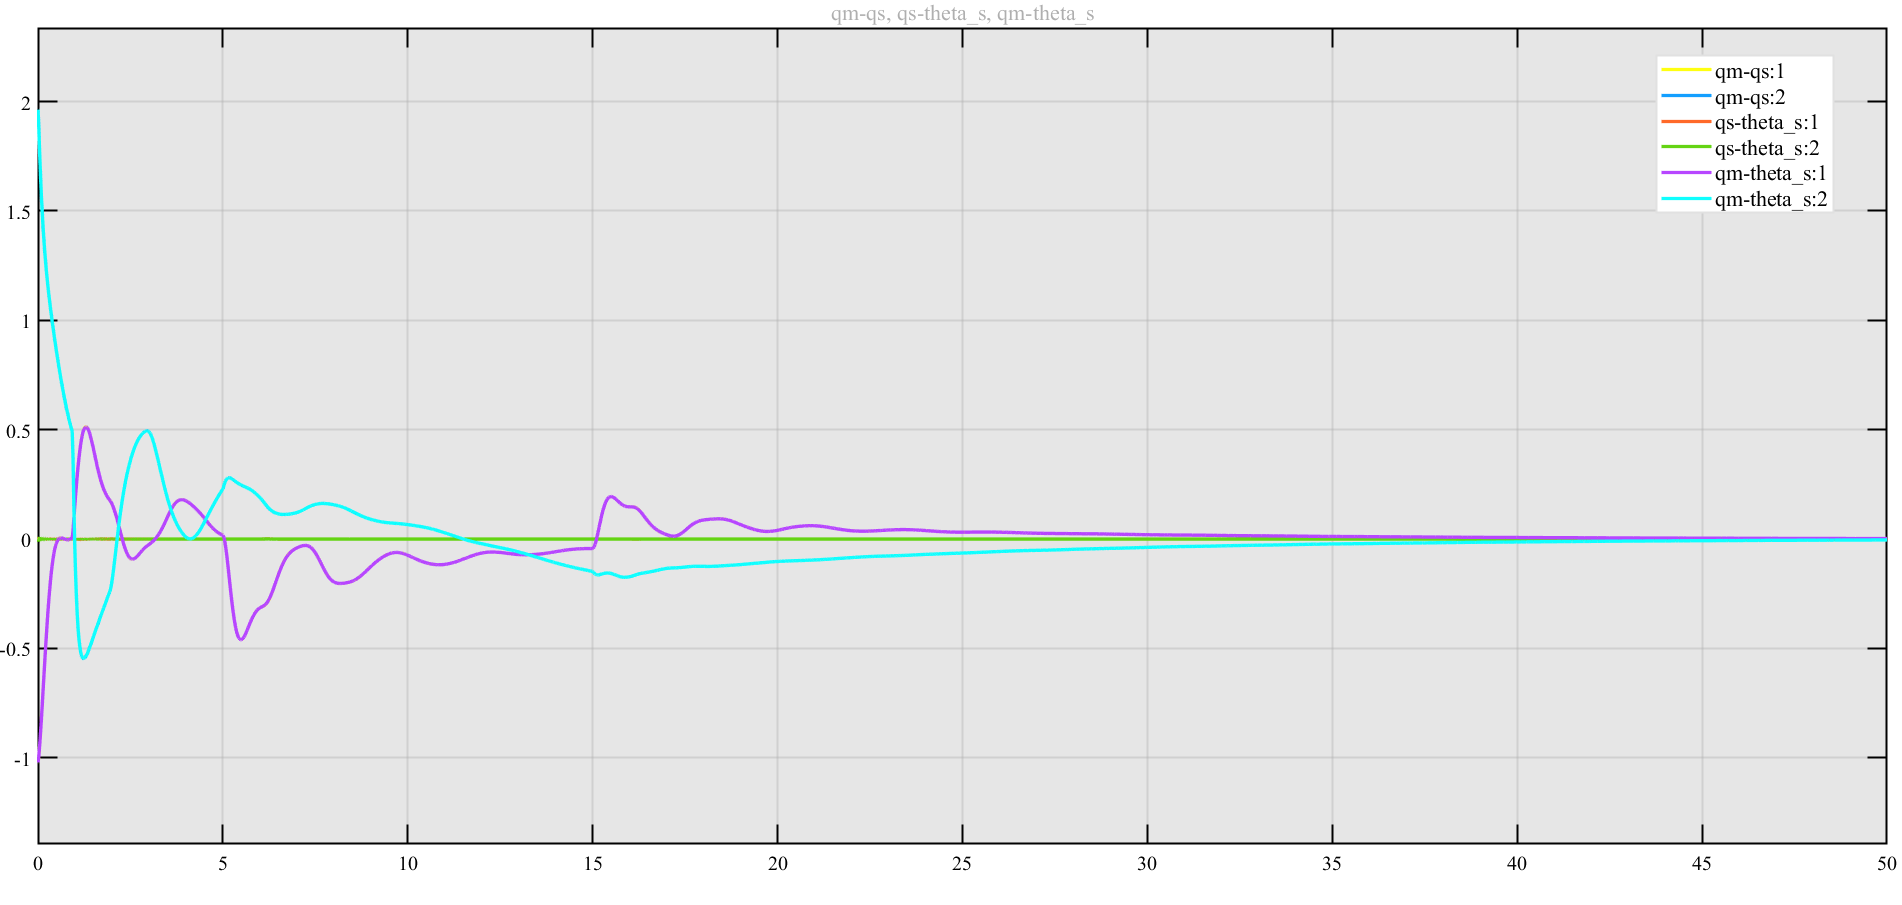
\includegraphics[width=0.95\textwidth]{fig/scope_vibration.png}
	\caption{柔性关节弹性变形响应}
	\label{fig:scope_vibration}
\end{figure}

为了分析柔性关节振动情况，本文选取电机转角与连杆转角之间的差值

\[
\Delta\theta=\theta-q
\]

作为柔性关节弹性变形量。

由图\ref{fig:scope_vibration}可知，在仿真开始阶段，由于控制输入突变以及柔性关节弹性作用，关节出现一定程度的振荡。随着控制器持续作用，振动幅值逐渐减小，并最终稳定在零附近。

说明控制器不仅能够保证机械臂的位置跟踪性能，而且能够增加系统阻尼，加快柔性关节振动衰减速度，有效降低弹性变形，提高机械臂运动稳定性。

此外，在整个仿真过程中，柔性关节变形始终保持在较小范围内，没有出现持续振荡现象，表明动力学模型具有较好的数值稳定性。

\subsubsection{控制输入分析}

控制器输出力矩如图\ref{fig:scope_torque}所示。

\begin{figure}[htbp]
	\centering
	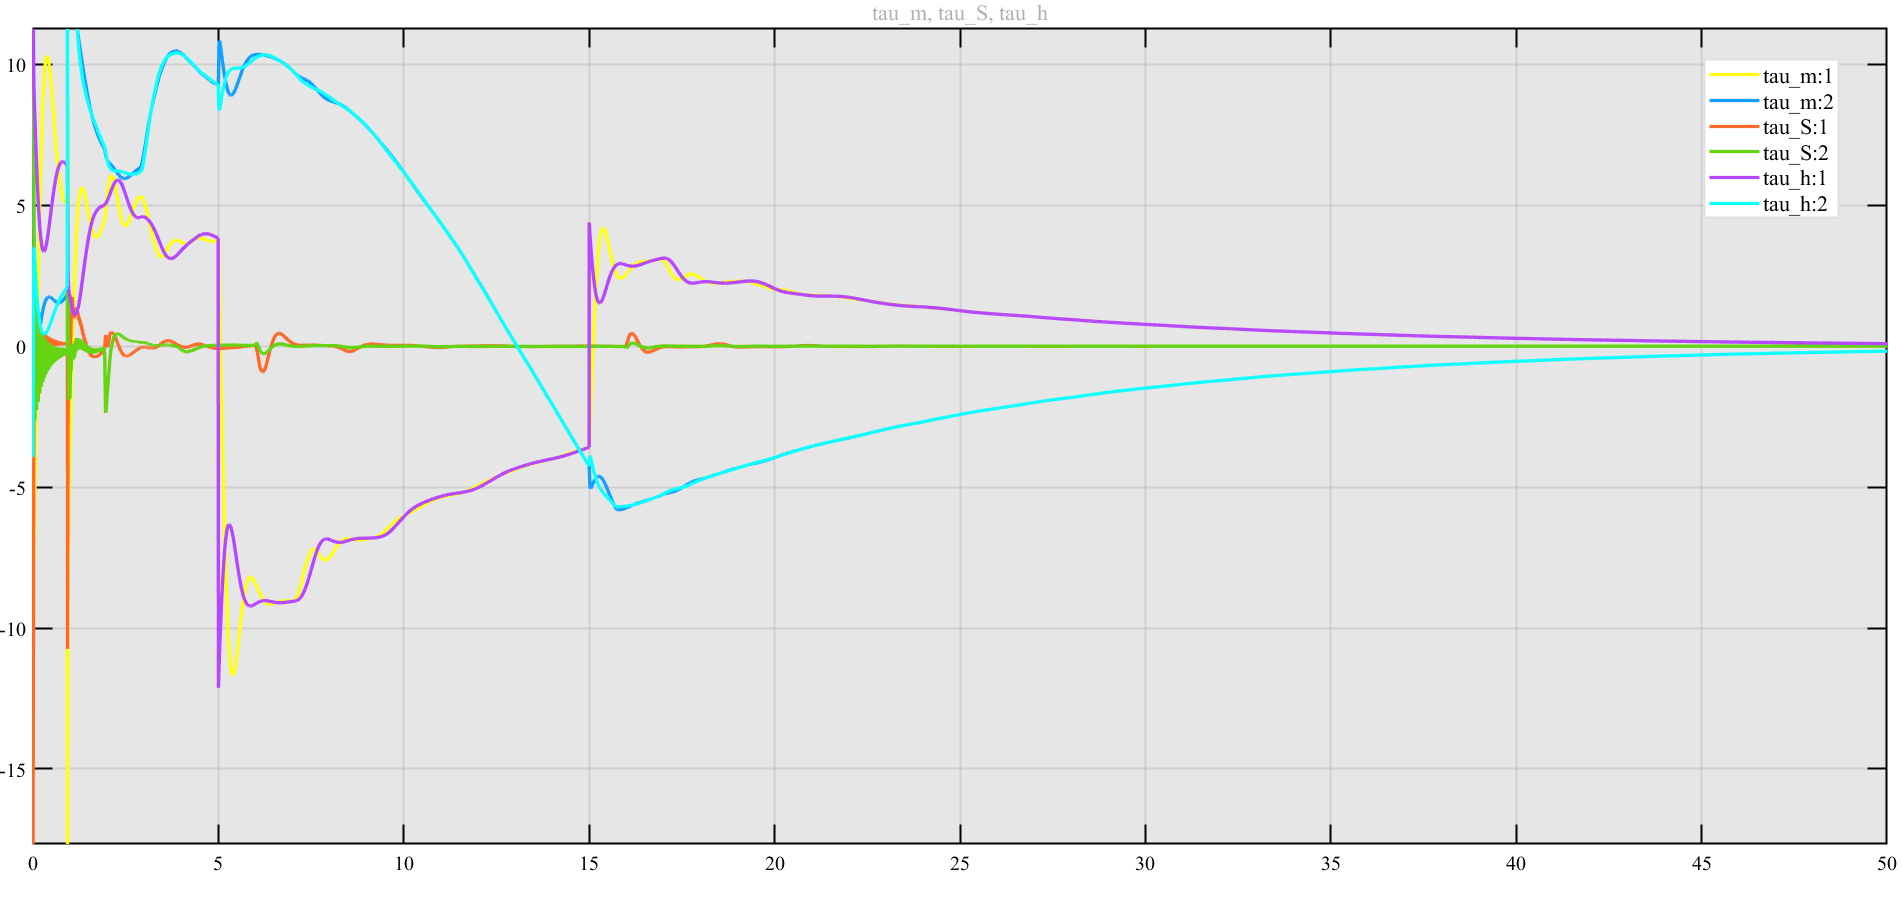
\includegraphics[width=0.95\textwidth]{fig/scope_torque.png}
	\caption{控制输入响应}
	\label{fig:scope_torque}
\end{figure}

由图\ref{fig:scope_torque}可以看出，在仿真初始阶段，由于机械臂需要克服初始误差，控制器输出较大的驱动力矩；随着机械臂逐渐接近参考轨迹，控制输入逐渐减小，并最终保持在较为稳定的范围内。

整个控制过程中，驱动力矩变化连续，没有出现明显的高频抖动和剧烈波动，说明控制器输出平滑，能够满足柔性关节机械臂驱动系统的控制要求。

同时，由于PD控制器具有一定阻尼作用，在保证快速响应的同时，有效避免了控制输入过大引起的机械振动，提高了系统运行稳定性。

\subsection{本章小结}

仿真结果表明，所建立的两连杆柔性关节机械臂动力学模型能够较好地描述机械臂的动态特性。基于PD控制器的控制策略能够实现机械臂关节对参考轨迹的准确跟踪，并有效抑制柔性关节产生的弹性振动。

从位置响应、柔性关节变形以及控制输入等仿真结果可以看出，机械臂具有较好的动态性能和控制稳定性，为后续参数辨识及实验平台验证奠定了基础。

\section{结论与展望}

本实验完成了两连杆柔性关节机械臂的动力学建模、参数辨识与PD控制器设计。仿真结果验证了模型准确性和控制器的有效性。未来可进一步引入自适应控制以提升鲁棒性。

	%%----------- 参考文献 -------------------%%
	\newpage
	\bibliographystyle{gbt7714-numerical}
	\bibliography{reference}
	
\end{document}